% Options for packages loaded elsewhere
\PassOptionsToPackage{unicode}{hyperref}
\PassOptionsToPackage{hyphens}{url}
%
\documentclass[
  12pt,
]{article}
\usepackage{amsmath,amssymb}
\usepackage{lmodern}
\usepackage{ifxetex,ifluatex}
\ifnum 0\ifxetex 1\fi\ifluatex 1\fi=0 % if pdftex
  \usepackage[T1]{fontenc}
  \usepackage[utf8]{inputenc}
  \usepackage{textcomp} % provide euro and other symbols
\else % if luatex or xetex
  \usepackage{unicode-math}
  \defaultfontfeatures{Scale=MatchLowercase}
  \defaultfontfeatures[\rmfamily]{Ligatures=TeX,Scale=1}
\fi
% Use upquote if available, for straight quotes in verbatim environments
\IfFileExists{upquote.sty}{\usepackage{upquote}}{}
\IfFileExists{microtype.sty}{% use microtype if available
  \usepackage[]{microtype}
  \UseMicrotypeSet[protrusion]{basicmath} % disable protrusion for tt fonts
}{}
\makeatletter
\@ifundefined{KOMAClassName}{% if non-KOMA class
  \IfFileExists{parskip.sty}{%
    \usepackage{parskip}
  }{% else
    \setlength{\parindent}{0pt}
    \setlength{\parskip}{6pt plus 2pt minus 1pt}}
}{% if KOMA class
  \KOMAoptions{parskip=half}}
\makeatother
\usepackage{xcolor}
\IfFileExists{xurl.sty}{\usepackage{xurl}}{} % add URL line breaks if available
\IfFileExists{bookmark.sty}{\usepackage{bookmark}}{\usepackage{hyperref}}
\hypersetup{
  pdftitle={Authority After the Tempest: Hurricane Michael and the 2018 Elections},
  pdfauthor={Kevin Morris; Peter Miller},
  hidelinks,
  pdfcreator={LaTeX via pandoc}}
\urlstyle{same} % disable monospaced font for URLs
\usepackage[margin=1in]{geometry}
\usepackage{longtable,booktabs,array}
\usepackage{calc} % for calculating minipage widths
% Correct order of tables after \paragraph or \subparagraph
\usepackage{etoolbox}
\makeatletter
\patchcmd\longtable{\par}{\if@noskipsec\mbox{}\fi\par}{}{}
\makeatother
% Allow footnotes in longtable head/foot
\IfFileExists{footnotehyper.sty}{\usepackage{footnotehyper}}{\usepackage{footnote}}
\makesavenoteenv{longtable}
\usepackage{graphicx}
\makeatletter
\def\maxwidth{\ifdim\Gin@nat@width>\linewidth\linewidth\else\Gin@nat@width\fi}
\def\maxheight{\ifdim\Gin@nat@height>\textheight\textheight\else\Gin@nat@height\fi}
\makeatother
% Scale images if necessary, so that they will not overflow the page
% margins by default, and it is still possible to overwrite the defaults
% using explicit options in \includegraphics[width, height, ...]{}
\setkeys{Gin}{width=\maxwidth,height=\maxheight,keepaspectratio}
% Set default figure placement to htbp
\makeatletter
\def\fps@figure{htbp}
\makeatother
\setlength{\emergencystretch}{3em} % prevent overfull lines
\providecommand{\tightlist}{%
  \setlength{\itemsep}{0pt}\setlength{\parskip}{0pt}}
\setcounter{secnumdepth}{5}
\usepackage{rotating}
\usepackage{setspace}
\newcommand{\beginsupplement}{\setcounter{table}{0}  \renewcommand{\thetable}{A\arabic{table}} \setcounter{figure}{0} \renewcommand{\thefigure}{A\arabic{figure}}}
\usepackage{lineno}
\linenumbers
\usepackage{booktabs}
\usepackage{longtable}
\usepackage{array}
\usepackage{multirow}
\usepackage{wrapfig}
\usepackage{float}
\usepackage{colortbl}
\usepackage{pdflscape}
\usepackage{tabu}
\usepackage{threeparttable}
\usepackage{threeparttablex}
\usepackage[normalem]{ulem}
\usepackage{makecell}
\usepackage{xcolor}
\ifluatex
  \usepackage{selnolig}  % disable illegal ligatures
\fi
\newlength{\cslhangindent}
\setlength{\cslhangindent}{1.5em}
\newlength{\csllabelwidth}
\setlength{\csllabelwidth}{3em}
\newenvironment{CSLReferences}[2] % #1 hanging-ident, #2 entry spacing
 {% don't indent paragraphs
  \setlength{\parindent}{0pt}
  % turn on hanging indent if param 1 is 1
  \ifodd #1 \everypar{\setlength{\hangindent}{\cslhangindent}}\ignorespaces\fi
  % set entry spacing
  \ifnum #2 > 0
  \setlength{\parskip}{#2\baselineskip}
  \fi
 }%
 {}
\usepackage{calc}
\newcommand{\CSLBlock}[1]{#1\hfill\break}
\newcommand{\CSLLeftMargin}[1]{\parbox[t]{\csllabelwidth}{#1}}
\newcommand{\CSLRightInline}[1]{\parbox[t]{\linewidth - \csllabelwidth}{#1}\break}
\newcommand{\CSLIndent}[1]{\hspace{\cslhangindent}#1}

\title{Authority After the Tempest: Hurricane Michael and the 2018 Elections}
\author{Kevin Morris\footnote{Researcher, Brennan Center for Justice at NYU School of Law, 120 Broadway Ste 1750, New York, NY 10271 (\href{mailto:kevin.morris@nyu.edu}{\nolinkurl{kevin.morris@nyu.edu}})} \and Peter Miller\footnote{Researcher, Brennan Center for Justice at NYU School of Law, 120 Broadway Ste 1750, New York, NY 10271 (\href{mailto:peter.miller@nyu.edu}{\nolinkurl{peter.miller@nyu.edu}})}}
\date{June 13, 2021}

\begin{document}
\maketitle
\begin{abstract}
Hurricane Michael made landfall in the Florida panhandle 27 days before the 2018 elections. In the aftermath, the governor of Florida issued Executive Order 18-283 granting election officials in 8 impacted counties the autonomy to loosen a variety of voting laws and consolidate polling places. We test the efficacy of the order using a novel research design to separate the weather effects of the hurricane on turnout from the administrative effects of actions taken by election officials. We show that the Executive Order was successful at eliminating much of the turnout decline following from the hurricane when counties maintained polling places in their planned, pre-election configuration, but voters in counties with many closed polling places were much more likely to abstain than shift to early or mail voting. We argue that natural disasters need not spell turnout disasters if administrators are able to avoid reducing the number of polling places available to voters.
\end{abstract}

\pagenumbering{gobble}
\pagebreak

\pagenumbering{arabic}
\doublespacing

\hypertarget{introduction}{%
\section*{Introduction}\label{introduction}}
\addcontentsline{toc}{section}{Introduction}

As the 2018 elections approached, an unanticipated---but not unprecedented---shape appeared on the Florida horizon: the Category 5 Hurricane Michael.\footnote{The category of the hurricane refers to the maximum sustained wind speed, according to the Saffir-Simpson hurricane wind scale. A Category 5 hurricane sustains winds greater than 157 miles per hour, as measured as the peak 1-minute wind at a height of 33 feet. See \url{https://www.nhc.noaa.gov/pdf/sshws.pdf}.} The hurricane made landfall on October 10, 27 days before the election, and would ultimately cause 16 deaths and 25 billion dollars in damage.\footnote{See \url{https://www.nhc.noaa.gov/data/tcr/AL142018_Michael.pdf}.} Would-be voters in the election were now faced with myriad disruptions to their daily lives; the direct effects of the weather, therefore, likely reduced turnout substantially as the recovery from the hurricane progressed. As professor emeritus Robert Montjoy told \emph{NPR} in the aftermath of the storm, ``Whether casting a ballot becomes a higher priority than cleaning out the basement, visiting someone in the hospital, or all the other demands\ldots You certainly expect a lower turnout for those reasons'' (\protect\hyperlink{ref-Parks2018}{Parks 2018}).

The storm also affected the administration of the election itself, as polling places were destroyed and potential mail voters found themselves temporarily residing at addresses other than those at which they were registered. The governor of Florida issued Executive Order 18-283\footnote{See \url{https://www.flgov.com/wp-content/uploads/2018/10/SLT-BIZHUB18101809500.pdf}.} as a means to counteract the widespread effects of the hurricane on October 18. Executive Order 18-283 sought to offset the administrative barriers to voting by allowing election administrators in 8 counties in Florida affected by the hurricane to flexibly respond to the damage wrought by the storm. Specifically, Executive Order 18-283 allowed administrators to add early voting locations; begin early voting 15 days before the general election (4 days after the Executive Order was issued), and continue until the day of the election; to accept vote-by-mail requests to addresses other than a voter's registered address; to send vote-by-mail ballots by forwardable mail; to deliver vote-by-mail ballots to electors or electors' immediate family members on election day without an affidavit; to relocate or consolidate polling places; and required poll watchers to be registered by the second Friday before the general election. The Executive Order covered Bay, Calhoun, Franklin, Gadsden, Gulf, Jackson, Liberty, and Washington Counties.

This paper sets out to answer a number of questions: what was the total depressive effect of the hurricane on turnout in the election? Did Executive Order 18-283 effectively offset the effects of the weather? More specifically, did easing mail-balloting and early voting rules reduce the impact of closed or moved polling places? We propose a novel research design to investigate these interrelated questions---what we are calling a double-matched, triple-difference model. We use a geographical regression discontinuity that takes advantage of the fact that voters on either side of the outermost borders of the counties covered by the Executive Order were treated to identical \emph{weather} effects from the hurricane, but that only some of them were further treated by the administrative changes allowed by the Executive Order. We strengthen the plausibility of this design by using a matching design to select voters subject only to the weather treatment that look very similar to those who received both treatments. By further matching each of these pairs of voters to registered voters elsewhere in the state---voters who were not impacted by Hurricane Michael---we decompose the weather and administrative effects of the hurricane on turnout.

Our results paint a complex picture. On the one hand, we find that voters who were subjected to worse weather turned out at lower rates after we control for the polling place consolidation of the county they lived in. We find, however, that the number of polling places a county eliminated had a much larger effect on turnout than the amount of rainfall voters experienced. In fact, at the very edges of the counties covered by the Executive Order we find no weather effect at all---but that the turnout of voters who lived just inside the covered counties was reduced on average by nearly 2 percentage points. The heterogeneity in county-level polling place consolidation makes clear that this was a function of polling place consolidation. Moreover, we show that voters who suddenly had to travel much further than planned to a polling place did not seamlessly shift to loosened mail voting options, but were instead substantially more likely to abstain from voting altogether. In short, counties that avoided polling place closures saw negligible turnout effects, but where counties closed a majority of their polling places, loosened restrictions did little to offset those costs.

As hurricanes grow increasingly frequent and intense due to climate change, understanding how to manage elections to ensure that they remain equitable and accessible will only become more important. While this is abundantly clear in the United States, where federal elections are held in early November, it is equally true for democracies around the globe. Typhoon Lan, for instance, disrupted Japanese elections in 2017 as we discuss below. While conducting an election under such circumstances is never easy, our results indicate that major turnout losses can perhaps be avoided if polling places remain open.

\hypertarget{literature-review}{%
\section*{Literature Review}\label{literature-review}}
\addcontentsline{toc}{section}{Literature Review}

The institutional and weather conditions of Hurricane Michael make it ripe for studying the interactive effects of severe weather, polling place siting, and administrative regimes. Indeed, the heterogeneity of county-level responses to the Executive Order allows us to precisely test the effects of these choices. Understanding these relationships will be of key importance in the coming years as climate change leads to increasingly strong storms (\protect\hyperlink{ref-Mann2006}{Mann and Emanuel 2006}). This is doubly true in the American context, where federal elections are held at the end of hurricane season. Although little work has explored how these effects interact, we here consider how Florida's permissive early voting regime, the Executive Order's allowance of polling place consolidation, and severe weather might have collectively structured turnout in 2018. Our general conclusion from the extant literature is that, early voting could have likely served as a ``relief valve'' on the pressures introduced by the inclement weather, but that polling place consolidation likely had major, negative turnout effects.

\hypertarget{early-voting-and-inclement-weather}{%
\subsection*{Early Voting and Inclement Weather}\label{early-voting-and-inclement-weather}}
\addcontentsline{toc}{subsection}{Early Voting and Inclement Weather}

It is well established that inclement weather on election day reduces turnout in both the American (\protect\hyperlink{ref-Cooperman2017}{Cooperman 2017}; \protect\hyperlink{ref-Hansford2010}{Hansford and Gomez 2010}) and international context (\protect\hyperlink{ref-Rallings2003}{Rallings, Thrasher, and Borisyuk 2003}), especially in noncompetitive and general elections (\protect\hyperlink{ref-Gatrell2002}{Gatrell and Bierly 2002}; \protect\hyperlink{ref-Fraga2010}{Fraga and Hersh 2010}). A recent study based on Irish parliamentary elections indicates that this is especially true in densely populated areas (\protect\hyperlink{ref-Garcia-Rodriguez2020}{Garcia-Rodriguez and Redmond 2020}). Severe weather reduces turnout by increasing the opportunity cost of voting: driving to a polling place or, worse, waiting outside in line to vote is obviously much more costly in severe weather events. As the quote in the Introduction from professor emeritus Robert Montjoy makes evident, a natural disaster can increase burdens on households even if it strikes before election day, perhaps leaving them less likely to learn about the candidates, locate their polling place, and cast a ballot.

Although Floridians in the panhandle faced a Category 5 hurricane in 2018, the hurricane arrived against the backdrop of Florida's permissive early voting infrastructure. Since 2008, about 25\% of Floridians, on average, have cast their ballots early in-person, prior to election day.\footnote{This estimate is based on our analysis of Voter Registration Supplements to the Current Population Survey over six general elections between 2008 and 2018.} It seems plausible that this availability could have sufficiently reduced the cost of voting to offset some of the negative effects associated with the storm. While research on the impact of early in-person voting on turnout in non-emergency times has returned mixed results (see, for instance, \protect\hyperlink{ref-Ricardson1996}{Ricardson and Neeley 1996}; \protect\hyperlink{ref-Larocca2011}{Larocca and Klemanski 2011}; \protect\hyperlink{ref-Burden2014}{Burden et al. 2014}; \protect\hyperlink{ref-Kaplan2020}{Kaplan and Yuan 2020}), a growing body of literature suggests that the availability of early in-person voting might be important in the context of severe weather. One study in Sweden, for instance, found no significant turnout effects of rain on election day, which they attribute to Sweden's permissive early voting regime (\protect\hyperlink{ref-Persson2014}{Persson, Sundell, and Öhrvall 2014, 337}); voters were able to avoid an incoming storm by casting a ballot in advance.

Most relevant to our study of Hurricane Michael are the effects of Superstorm Sandy on turnout in the Northeastern US in 2012 and Typhoon Lan\footnote{Lan was the equivalent of a Category 4 hurricane, featuring wind speeds of between 130 and 156 miles per hour.} in the 2017 House of Representatives election in Japan. The typhoon made landfall the day after election day, though it appears voters behaved dynamically as the typhoon approached: voters were more likely to vote early, or earlier on the day of the election, as rainfall increased in prefectures in the path of the typhoon (\protect\hyperlink{ref-Kitamura2021}{Kitamura and Matsubayashi 2021}). Of course, we cannot know which individuals who voted early would have braved the storm and voted even in the absence of such an option, and which would have opted to stay home. Nevertheless, it is not unreasonable to assume that the availability of early voting allowed some voters to participate who would not have in worse weather.

The experience of Superstorm Sandy in the Northeastern United States in 2012, a storm whose political impacts have been studied by a number of scholars (\protect\hyperlink{ref-Lasala-Blanco2017}{Lasala-Blanco, Shapiro, and Rivera-Burgos 2017}; \protect\hyperlink{ref-Velez2013}{Velez and Martin 2013}), provides more evidence of the importance of early voting in the face of severe weather. Stein (\protect\hyperlink{ref-Stein2015}{2015, 69}) argues that turnout in counties impacted by Superstorm Sandy decreased by 2.8\% between 2008 and 2012---a full 2\% more than the rest of the country. He finds, however, that counties that provided for early in-person voting actually saw \emph{higher} turnout in 2012 than other comparable counties. It seems that, whatever questions remain about the impact of early in-person voting on turnout in normal times, that such an option may provide a way to recoup some of the lost turnout caused by a natural disaster.

\hypertarget{polling-place-consolidation}{%
\subsection*{Polling Place Consolidation}\label{polling-place-consolidation}}
\addcontentsline{toc}{subsection}{Polling Place Consolidation}

Even as Floridians had access to widespread early in-person voting in 2018, Hurricane Michael and Executive Order 18-283 allowed for and effected major polling place consolidation in the covered counties. In fact, just 61 of the planned 125 polling places were open across the 8 counties covered by the Executive Order. Understanding the impact of these consolidations in light of the hurricane is important for situating the anticipated effect of the storm on turnout---and, in particular, the effect of choices made by local election administrators under the flexibility granted by the Executive Order.

Voting rights advocates recently argued that polling place closures should be avoided in an emergency, even when vote-by-mail restrictions are loosened. While Hurricane Michael preceded the coronavirus pandemic, the arguments made in 2020 against widespread closures apply equally to closures from a hurricane. As \protect\hyperlink{ref-Macias2020}{Macías and Pérez} (\protect\hyperlink{ref-Macias2020}{2020}) at the Brennan Center for Justice argued, ``{[}m{]}any Americans do not have access to reliable mail delivery, and many do not have conventional mailing addresses for ballot delivery. Eliminating polling sites would completely disenfranchise these voters.'' The Center for American Progress made a similar argument, writing that ``{[}w{]}hile vote by mail is an option that works for many Americans, it is not a viable option for everyone. Specifically, eliminating all in-person voting options would disproportionately harm African American voters, voters with disabilities, American Indian and Alaska Native voters, and those who rely on same-day voter registration'' (\protect\hyperlink{ref-Root2020}{Root et al. 2020}). In other words, voting rights advocates argue not only that polling place closures in an emergency reduce turnout, but that the turnout reductions do not fall evenly across the electorate.

The scholarly literature bears this out. Although \protect\hyperlink{ref-Stein2015}{Stein} (\protect\hyperlink{ref-Stein2015}{2015}) argues that counties impacted by Superstorm Sandy that consolidated polling places saw \emph{higher} turnout than those that were affected but did not consolidate their polling places, this result is something of an outlier. The extant literature is consistent in its conclusion that polling place consolidation reduces turnout. Relocating or reducing the number of polling places reduces turnout by imposing new search and transportation costs on voters (\protect\hyperlink{ref-Brady2011}{Brady and McNulty 2011}). A moved polling place reduces turnout in a variety of electoral contexts (\protect\hyperlink{ref-Cantoni2020}{Cantoni 2020}), including local elections (\protect\hyperlink{ref-McNulty2009}{McNulty, Dowling, and Ariotti 2009}; \protect\hyperlink{ref-Haspel2005}{Haspel and Knotts 2005}) as well as national contests (\protect\hyperlink{ref-Kropf2012}{Kropf and Kimball 2012}). Absentee voting is more likely as the distance to the polls increases, but this effect is not large enough to offset the decrease from consolidation itself (\protect\hyperlink{ref-Brady2011}{Brady and McNulty 2011}; \protect\hyperlink{ref-Dyck2005}{Dyck and Gimpel 2005}).

Although there has been little work on the effect of polling place consolidation on turnout in the face of a storm, recent work indicates that last-minute polling place consolidation reduced turnout during the Covid-19 pandemic in 2020. During the April 2020 primary election in Milwaukee, Wisconsin, the municipality went from 182 to just 5 polling places. \protect\hyperlink{ref-Morris2021}{Morris and Miller} (\protect\hyperlink{ref-Morris2021}{2021}) shows that this consolidation had major, negative turnout effects, even though Wisconsin has a robust absentee voting regime. They conclude: ``Even as many voters transition to vote-by-mail in the face of a pandemic, polling place consolidation can still have disenfranchising effects'' (\protect\hyperlink{ref-Morris2021}{Morris and Miller 2021, 13}). While polling place closures and movements seem to impose costs on voters and reduce turnout even under the best of circumstances, it seems possible that these costs are much higher when coupled with the other demands on voters' time imposed by emergency situations---even when other alternatives such as absentee voting are readily available.

Grounding our analyses of the effects of Hurricane Michael gives us some expectations as to how the hurricane altered voting behavior. We expect the direct, weather-related effects of the hurricane reduced turnout. The administrative effects---that is, the turnout effects arising from decisions made by election administrators under the latitude granted by the Executive Order---will push in opposite directions. On the one hand, consolidated polling places likely imposed costs on voters, reducing turnout above-and-beyond the direct effects of weather. On the other hand, the relief valve offered by early voting may recover \emph{some but not all} of these displaced voters. This is, of course, not to claim that the local officials in the path of the hurricane sought to reduce turnout. Rather, the work of administering an election---even under the best of circumstances---is a complex, interconnected process involving multiple actors (\protect\hyperlink{ref-Hale2015}{Hale, Montjoy, and Brown 2015}; \protect\hyperlink{ref-Brown2019}{Brown, Hale, and King 2019}).

\hypertarget{research-design-and-expectations}{%
\section*{Research Design and Expectations}\label{research-design-and-expectations}}
\addcontentsline{toc}{section}{Research Design and Expectations}

We expect that Hurricane Michael depressed turnout in the 2018 midterm election via two causal mechanisms: weather effects and administrative effects. By weather effects, we mean the direct costs imposed on voters, such as destroyed or damaged property and temporary relocation. Administrative effects refer to the turnout effects of the choices made by election administrators udner to the discretion afforded by Executive Order 18-283. Throughout our analyses, we examine the effects of the hurricane on voters registered as of the 2018 election. Put differently, we do not test the turnout of \emph{eligible citizens}. Conditioning turnout on registration status raises important questions when the treatment might influence registration (see \protect\hyperlink{ref-Nyhan2017}{Nyhan, Skovron, and Titiunik 2017}). That is likely the case here: as we demonstrate in the Supplementary Information, it seems probable that Hurricane Michael reduced registrations in the days before the registration deadline. Our models cannot capture these turnout effects; as such, our estimated negative treatment effects should be considered conservative, as we are not measuring the turnout of individuals whose registration---and subsequent participation---was impeded by the storm.

\hypertarget{estimating-the-overall-effects-of-the-hurricane}{%
\subsection*{Estimating the Overall Effects of the Hurricane}\label{estimating-the-overall-effects-of-the-hurricane}}
\addcontentsline{toc}{subsection}{Estimating the Overall Effects of the Hurricane}

We begin by testing the average marginal effect (AME) of Hurricane Michael on turnout. The AME is the net effect of both the weather and the administrative effects on individual-level turnout. Our central identification strategy involves the use of difference-in-differences models. We use voter-file data from L2 Political to estimate individual-level turnout and to control for individual-level characteristics and the latitude and longitude of each voter's residential address. L2 uses models to predict individual race / ethnicity and voters' sex but these characteristics are available in self-reported form in the raw voter-file available from the state; as such, we pull sex and race / ethnicity from the publicly available voter file. The L2 data is based on the February 8, 2019, version of the raw voter file, the same file from which we pull race / ethnicity and sex.

In addition to the individual-level characteristics from the voter file, we also proxy each voter's exposure to Hurricane Michael using rainfall data. The National Oceanic and Atmospheric Administration (NOAA) makes daily rainfall data available for some 13,000 stations around the United States. We use the \texttt{rnoaa} (\protect\hyperlink{ref-Chamberlain2021}{Chamberlain 2021}) package to measure the amount of rain that fell between October 10 and November 6 in 2018 (relative to the average rainfall in that period from 2000 to 2017) at each weather station in the country. Voters' individual exposure to rainfall is calculated as the average of the three closest weather stations, inversely weighted by distance.

Finally, we incorporate information garnered from public records requests sent to each of the 8 treated counties. Although the counties did not, by-and-large, take advantage of the opportunity to add early voting days granted by the Executive Order (no county increased the number of days by more than 2), some counties did reduce the number of polling places. Three counties (Calhoun, Gadsden, and Liberty) closed no polling places, while a fourth (Franklin) actually added an additional polling place. The other four covered counties cut the number of polling places by at least two-thirds. We leverage this heterogeneity to explore the effect of closed polling places on turnout, and expect the turnout effect of the storm was lower (that is, less negative) in the counties where more polling places were open. In the Supplementary Information we include a table detailing the number of polling places and days of early voting in each covered county.

By comparing historical and 2018 turnout for voters in the counties hit by the storm to historical and 2018 turnout of voters elsewhere in the state, we can estimate the AME of the storm on turnout. To ensure a high-quality difference-in-differences specification, we do not include all untreated voters in our control group; rather, we genetically match (\protect\hyperlink{ref-Sekhon2011}{Sekhon 2011}) each treated voter with five untreated voters along a battery of individual- and neighborhood-level characteristics, including past turnout and vote mode. Untreated voters who do not serve as matches are excluded from our models. Although it may seem counterintuitive to exclude data from our models, this matching procedure substantially improves the parallel trends assumptions necessary for a rigorous difference-in-differences analysis (\protect\hyperlink{ref-Sekhon2009}{Sekhon 2009, 496}; \protect\hyperlink{ref-Imai2020}{Imai, Kim, and Wang 2020}). As we show in the Supplementary Information, our estimated AME is robust to a variety of different pre-processing and modeling choices.

This design allows us to test our first hypothesis:

\textbf{Hypothesis 1:} Turnout among voters in the eight treated counties was depressed in the 2018 election relative to voters in untreated counties. We expect that the negative AME will be larger in counties that closed more polling places in response to the Executive Order, and where the relative rainfall was higher.

\hypertarget{decomposing-weather-and-administrative-effects}{%
\subsection*{Decomposing Weather and Administrative Effects}\label{decomposing-weather-and-administrative-effects}}
\addcontentsline{toc}{subsection}{Decomposing Weather and Administrative Effects}

To estimate the administrative effect on turnout, we must control for the weather effects encountered by each voter. To do so, we leverage the somewhat arbitrary borders of counties in the Florida Panhandle, an approach similar to that adopted in a different context by \protect\hyperlink{ref-Walker2019}{Walker, Herron, and Smith} (\protect\hyperlink{ref-Walker2019}{2019}). This is often referred to as a geographical regression discontinuity (\protect\hyperlink{ref-Keele2015b}{Keele and Titiunik 2015}). There is no reason to believe that the effects of a hurricane would change dramatically along county borders. We assume, therefore, that voters who lived nearby one another, but on either side of a county border, faced the same weather issues during the 2018 election. Put differently, these voters were identically ``treated'' by the weather effects of the hurricane. Within a narrow buffer around the county border, we can conceive of a voter's county as effectively randomly assigned. Any observed turnout differential, therefore, is attributable \emph{not} to the weather, but the administrative effects of the county in which they happen to live. While all these voters were ``treated'' by the hurricane, only those in the covered counties also received the administrative treatment arising from the Executive Order.

Of course, self-selection around a geographic boundary is entirely possible; as such, conceiving of the administrative boundary as a quasi-random assignment is perhaps too strong of an assumption. Treated and control voters, despite living very near to one another, might differ in meaningful ways. To address this potential problem, we adopt the technique developed by \protect\hyperlink{ref-Keele2015a}{Keele, Titiunik, and Zubizarreta} (\protect\hyperlink{ref-Keele2015a}{2015}) by also matching voters on either side of the boundary according to their historical turnout and vote mode. To strengthen the plausibility that these two sets of voters were identically treated by the weather, we also match on each voter's relative rainfall.

By comparing the 2018 turnout of these voters, we can identify the administrative effect of the Executive Order on turnout for the administratively treated voters living within the buffer around the border. By further comparing the turnout of these voters to (matched) voters elsewhere in the state, we can also estimate the weather effects of the storm. We call this a double-matched triple-differences (or difference-in-difference-in-differences) specification. We lay out the specific steps below.

We begin by constructing our set of voters who received an administrative treatment. These voters include all registered voters who live in a county covered by the Executive Order and within 2.5 miles of a bordering, uncovered county (See Figure \ref{fig:map}). Each treated voter is then matched to one voter who lives in an uncovered county, but within 2.5 miles of a covered county. All of these voters were treated by the weather, but only those in the covered counties were also treated by the administrative changes. Although Calhoun, Franklin, and Gulf Counties were covered by the Executive Order, no voters in these counties live within 2.5 miles of an uncovered county; as such, no voters from these counties are included in these models.

\begin{figure}[h]

{\centering 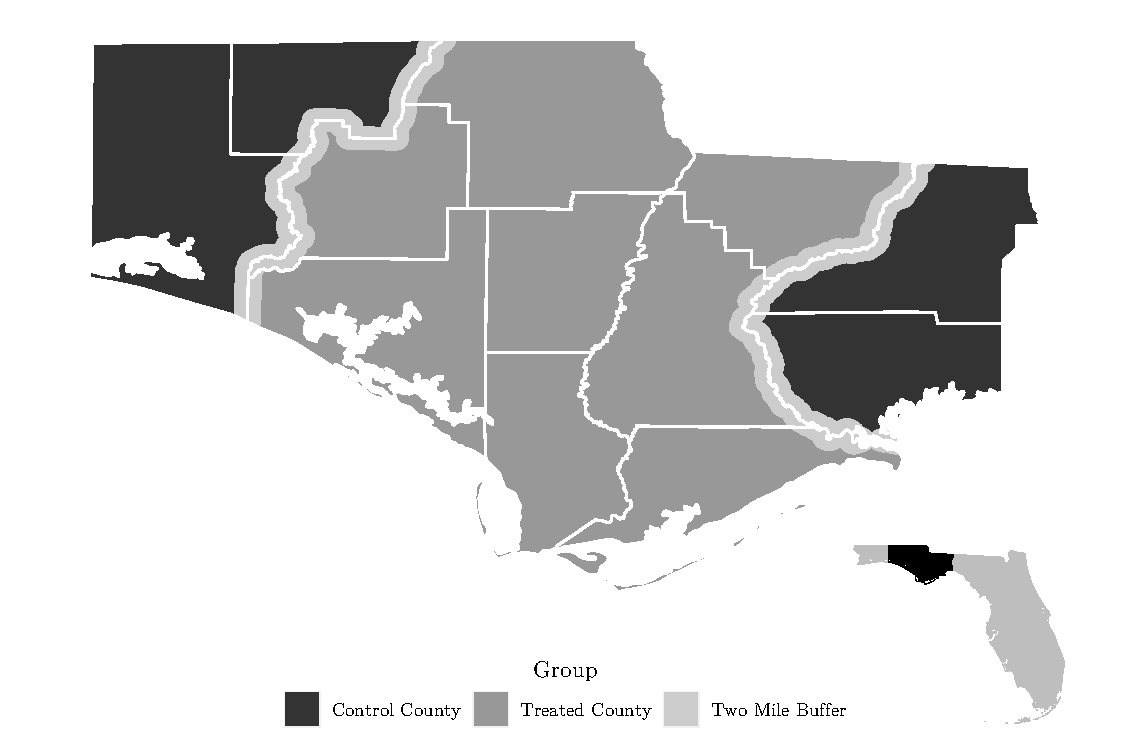
\includegraphics{hurricane_michael_files/figure-latex/map-chunk-1} 

}

\caption{\label{fig:map}Treated and Control Counties with 2.5 Mile Buffer}\label{fig:map-chunk}
\end{figure}

Each of these voters is subsequently matched to five voters elsewhere in the state---that is to say, voters who received neither a weather treatment \emph{nor} an administrative one. This exercise is the second match, and the matches are our control voters.

Table \ref{tab:groups} summarizes the treatment status of our three groups of voters.

\begin{singlespace}
\begin{table}[H]

\caption{\label{tab:groups-treat}\label{tab:groups} Treatment Status for Selected Voters}
\centering
\begin{tabular}[t]{>{\raggedright\arraybackslash}p{15em}ll}
\toprule
\multicolumn{1}{c}{ } & \multicolumn{2}{c}{Treatment Received} \\
\cmidrule(l{3pt}r{3pt}){2-3}
Group & Administrative & Weather\\
\midrule
\cellcolor{gray!6}{Voters in Covered Counties} & \cellcolor{gray!6}{Yes} & \cellcolor{gray!6}{Yes}\\
Voters in Uncovered Counties in Panhandle & No & Yes\\
\cellcolor{gray!6}{Voters Elsewhere} & \cellcolor{gray!6}{No} & \cellcolor{gray!6}{No}\\
\bottomrule
\end{tabular}
\end{table}
\end{singlespace}

Having constructed our pool of voters, we run a triple-differences model. This triple-differences model is, in effect, two simultaneous difference-in-differences models. The model estimates whether 2018 was associated with depressed turnout for voters treated only by the weather vis-à-vis the controls who received no treatment. Because these treated voters lived in counties not covered by the Executive Order, we assume that they faced no administrative effects from the storm. Any observed difference between these groups is therefore the weather effect for all voters treated by the weather, regardless of whether they received an additional, administrative treatment.

The model also estimates turnout differences between voters treated by the weather and administrative effects, and those treated only by the weather. Because we assume these closely-located voters faced identical weather effects, any difference between them is the administrative effect on turnout of their county's response to the Executive Order.

The double-matched triple-differences model allows us to test our second and third hypotheses:

\textbf{Hypothesis 2:} We expect that the hurricane had negative weather effects for voters who lived just outside of covered counties.

\textbf{Hypothesis 3:} We expect that the administrative effect will be largely driven by the number of polling places each county consolidated, other things equal. Where many polling places were closed we anticipate a large, negative administrative effect (\protect\hyperlink{ref-Morris2021}{Morris and Miller 2021}). In contrast, where most polling places remained open, we expect small negative or small positive administrative effects.

In short, our empirical strategy incorporates matching, difference-in-differences, and a regression discontinuity, three powerful tools for establishing causality. As we demonstrate in the Supplementary Information, our estimated administrative treatment is robust to specifications including a county-linear time trends, and without any matching at all.

\hypertarget{vote-mode}{%
\subsection*{Vote Mode}\label{vote-mode}}
\addcontentsline{toc}{subsection}{Vote Mode}

After estimating the double-matched triple-differences model, we turn to vote-mode within the treated counties. To test whether polling place closures allowed under the Executive Order shifted vote mode from in-person to either early or mail voting in the treated counties, we begin by calculating how far each voter lived from the closest planned polling place, and how far she lived from the closest polling place that was actually open on election day. Using the registered voter file, we can tell not only \emph{whether} a voter participated, but also \emph{how} they participated. Using a multinomial logistic regression, we test whether the difference between the planned and actual distance-to-polling-place were associated with vote-mode in 2018. This specification allows us to test our final hypothesis:

\textbf{Hypothesis 4}: As the difference between the actual and planned distance to the closest polling place increased for voters, they were more likely to vote absentee and to abstain from voting, all else being held equal.

\hypertarget{results}{%
\section*{Results}\label{results}}
\addcontentsline{toc}{section}{Results}

\hypertarget{overall-turnout-effects}{%
\subsection*{Overall Turnout Effects}\label{overall-turnout-effects}}
\addcontentsline{toc}{subsection}{Overall Turnout Effects}

We begin by matching each registered voter in the eight treated counties to five untreated voters elsewhere in the state using a nearest neighbor approach. We use a genetic algorithm to determine the weight each characteristic should receive for the matching procedure (\protect\hyperlink{ref-Sekhon2011}{Sekhon 2011}).\footnote{Due to computing constraints, the matching weights were constructed using a one percent random sample stratified by treatment status. The weights derived from the genetic algorithm are then used to perform the nearest-neighbor match for all treated voters.} The individual-level characteristics come directly from L2 and the registered voter file. The two neighborhood-level characteristics included---median income and share of the population with some collegiate education---are estimated at the block group level, and come from the ACS 5-year estimates ending with 2018. Ties are randomly broken, and matching is done with replacement.

Although the treated counties were at the center of the storm, nearby counties might have also been negatively impacted by the storm. Therefore, voters who live in the counties that border the treated counties are excluded as potential controls. These include Walton, Holmes, Wakulla, and Leon Counties. According to public records requests we filed, these counties did not reduce polling places or early voting days because of the hurricane. While they received no administrative treatment, we exclude them because of their potential weak weather treatment.

Table \ref{tab:full-bal} demonstrates the results of this matching procedure. As Table \ref{tab:full-bal} makes clear, voters in the affected counties were considerably more likely to be white and identify as Republicans, and live in lower-income neighborhoods, than voters in the rest of the state. The post-match control group, however, looks substantially similar to the treated voters. Though the matching process included historical vote mode, these are not included in Table \ref{tab:full-bal} but Figure \ref{fig:full-to} shows that the procedure was effective at reducing historical differences between the treated and potential control voters.

\begin{singlespace}
\begin{table}[!h]

\caption{\label{tab:balance-tab-full}\label{tab:full-bal} Balance Table for Statewide Matching}
\centering
\resizebox{\linewidth}{!}{
\begin{tabular}[t]{lllll}
\toprule
\multicolumn{1}{c}{ } & \multicolumn{2}{c}{Means: Unmatched Data} & \multicolumn{2}{c}{Means: Matched Data} \\
\cmidrule(l{3pt}r{3pt}){2-3} \cmidrule(l{3pt}r{3pt}){4-5}
 & Treated & Control & Treated & Control\\
\midrule
\% White & 76.5\% & 62.3\% & 76.5\% & 76.5\%\\
\% Black & 17.1\% & 13.1\% & 17.1\% & 17.1\%\\
\% Latino & 2.1\% & 17.4\% & 2.1\% & 2.1\%\\
\% Asian & 1.0\% & 2.0\% & 1.0\% & 1.0\%\\
\% Female & 52.5\% & 52.4\% & 52.5\% & 52.5\%\\
\% Male & 45.8\% & 44.9\% & 45.8\% & 45.8\%\\
Age & 52.2 & 52.5 & 52.2 & 52.2\\
\% Democrat & 39.2\% & 37.1\% & 39.2\% & 38.5\%\\
\% Republican & 43.6\% & 35.0\% & 43.6\% & 41.7\%\\
\% with Some College & 69.0\% & 75.1\% & 69.0\% & 69.0\%\\
Median Income & \$50,643 & \$62,941 & \$50,643 & \$50,727\\
Registration Date & 2002-03-13 & 2004-10-17 & 2002-03-13 & 2002-04-03\\
\bottomrule
\end{tabular}}
\end{table}
\end{singlespace}

Figure \ref{fig:full-to} plots the turnout in the past few elections for our treated and control voters. The left-hand panel shows the turnout of all voters registered in 2018. In the right-hand panel, we plot the turnout of treated voters and only their controls. As Figure \ref{fig:full-to} makes clear, turnout in the treated counties was consistently higher than the rest of the state---until 2018, when the hurricane hit. In the right-hand panel, we see that there was a substantial, negative treatment effect in 2018.

\begin{figure}[h]

{\centering 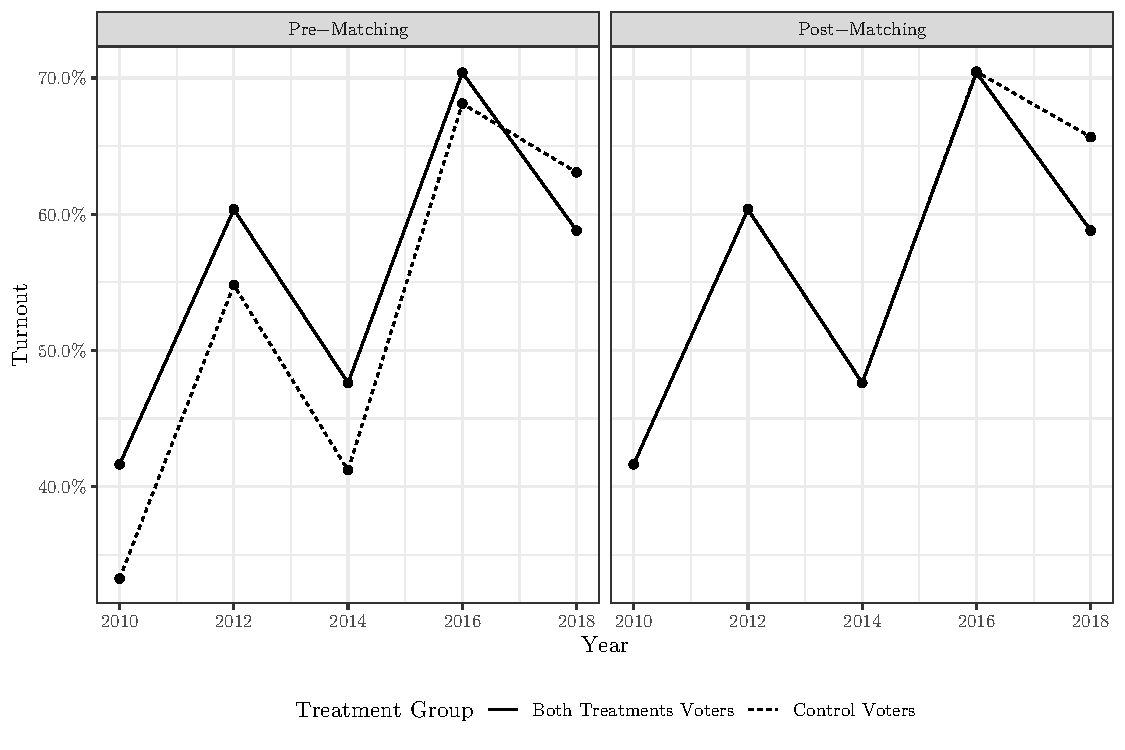
\includegraphics{hurricane_michael_files/figure-latex/full-to-chunk-1} 

}

\caption{\label{fig:full-to}General Election Turnout for Voters Covered by Executive Order and Their Controls, 2010 -- 2018}\label{fig:full-to-chunk}
\end{figure}

Table \ref{tab:full-dind} formalizes the right-hand panel of Figure \ref{fig:full-to} into a differences-in-differences regression. We employ an ordinary least squares specification. The dependent variable takes the value 1 if a voter cast a ballot in a given year, and 0 if she did not. In each model, \emph{Treated × 2018} estimates the average marginal effect of Hurricane Michael on turnout for treated voters. Model 2 also includes the characteristics on which the voters were matched. Model 3 adds a measure for congressional district competitiveness. Because this variable is ``downstream'' of treatment---that is to say, the effect of the hurricane could have impacted the competitiveness of certain races---it is not included in the first two models. It should be noted that each of the treated voters lived in uncontested congressional districts.

In model 4, we allow for the possibility that the treatment effect was different where the hurricane had greater intensity. In this model, \emph{Covered by EO × 2018 × Relative Rainfall} allows the treatment effect to vary based on our proxy for hurricane strength. Finally, in model 5, we ask whether the treatment effect was different in counties where fewer polling places were open (\emph{Covered by EO × 2018 × Share of Expected Polling Places Open}). Model 5 includes controls for hurricane strength to tease apart the effect of polling place closures from hurricane strength. In models 4 and 5, control voters are assigned the rain and county polling place values of their treated voter. While the regressions include the full set of uninteracted and interaction terms, we display only these variables' impact on the treatment estimate in table. In each model, robust standard errors are clustered at the level of the match (\protect\hyperlink{ref-Abadie2020}{Abadie and Spiess 2020}).

\begin{singlespace}
\input{"../temp/dind_full.tex"}
\end{singlespace}

The coefficient on \emph{Covered by EO × 2018} in Table \ref{tab:full-dind} indicates that Hurricane Michael had a substantial depressive effect in 2018 among the treated voters. Models 1 -- 3 indicate that the hurricane reduced turnout in the treated counties by roughly 6.6 percentage points. Multiplied across the nearly 200,000 registered voters in the treated counties indicates that some 13,000 ballots went uncast due to the hurricane, a major effect in a year when a statewide senate race was decided by 10,033 votes.

Model 4 indicates that the turnout effect was not moderated by the strength of the hurricane. It should be noted, however, that there is not a tremendous amount of variation in relative rainfall among treated voters: the interquartile range for rainfall relative to the historical average stretches from 174\% to 200\%. Model 5 makes clear that the treatment effect was highly moderated by the share of polling places each county had to close. The estimated treatment effect ranges from -9.4 percentage points in Bay County (where 6 of 44 polling places were open, and the rainfall was 184\% of normal) to a \emph{positive} treatment of 4.7 percentage points in Franklin County, where 8 polling places were open compared to just 7 planned ones (and rainfall was just 120\% of normal). As we demonstrate in the Supplementary Information, county-specific treatment effects corroborate the finding that polling place closures had a \emph{far larger} effect on turnout than relative rainfall---and that there was apparently a positive AME in Franklin County. In short, Table \ref{tab:full-dind} indicates that the negative turnout effects of a Category 5 hurricane that strikes weeks before an election can be mitigated by avoiding polling place consolidation.

\hypertarget{identifying-administrative-effects}{%
\subsection*{Identifying Administrative Effects}\label{identifying-administrative-effects}}
\addcontentsline{toc}{subsection}{Identifying Administrative Effects}

As discussed above, our primary strategy for isolating the administrative effects of the hurricane on turnout involves leveraging random assignment around county borders in the Florida panhandle in a double-matched triple-differences specification. Each voter inside the buffer in a covered county is matched with one voter in the buffer in an uncovered county, once again using a genetic matching algorithm (\protect\hyperlink{ref-Sekhon2011}{Sekhon 2011}). Ties are broken randomly, and matching is done with replacement.

In some cases, voters on either side of the border are in different congressional districts. This would pose a problem if these races were contested thanks to the potentially mobilizing effects of U.S. House races, but the entire buffer falls in uncontested congressional districts. This means that treated and untreated voters are not facing differential mobilization from congressional races. In constructing our full set of voters treated by weather effects, equalizing individual-level exposure to Hurricane Michael is of paramount importance. As such, in this first match, we include only historical vote mode, voters' relative rainfall, and latitude and longitude. This ensures that the voters treated by weather and administrative effects and those treated only by the weather will have similar past turnout trends and live near one another.

After matching, these pairs of voters live an average of about 3.6 miles from one another. Importantly, the relative rainfall faced by the two groups is virtually identical: while rainfall during the period was 164\% of normal for the voters outside the covered counties, it was 167\% of normal for the voters inside the covered counties. We consider these differences sufficiently small to assume that, on average, paired voters were faced with identical weather effects.

Once our full set of voters exposed to weather effects has been identified, each of these voters is matched with five other voters that lived in neither the covered nor the immediately surrounding counties. This matching procedure follows the same steps detailed in the Overall Turnout Effects section of this paper. Table \ref{tab:balance-secondary} presents the results of the secondary match. We improve along all characteristics.

\begin{singlespace}
\begin{table}[!h]

\caption{\label{tab:balance-tab-ll2}\label{tab:balance-secondary} Balance Table for Secondary Match}
\centering
\resizebox{\linewidth}{!}{
\begin{tabular}[t]{lllll}
\toprule
\multicolumn{1}{c}{ } & \multicolumn{2}{c}{Means: Unmatched Data} & \multicolumn{2}{c}{Means: Matched Data} \\
\cmidrule(l{3pt}r{3pt}){2-3} \cmidrule(l{3pt}r{3pt}){4-5}
 & Treated & Control & Treated & Control\\
\midrule
\% White & 73.4\% & 62.3\% & 73.4\% & 73.4\%\\
\% Black & 22.6\% & 13.1\% & 22.6\% & 22.6\%\\
\% Latino & 1.0\% & 17.4\% & 1.0\% & 1.0\%\\
\% Asian & 0.3\% & 2.0\% & 0.3\% & 0.3\%\\
\% Female & 53.1\% & 52.4\% & 53.1\% & 53.1\%\\
\% Male & 45.6\% & 44.9\% & 45.6\% & 45.6\%\\
Age & 53.3 & 52.5 & 53.3 & 53.2\\
\% Democrat & 45.6\% & 37.1\% & 45.6\% & 44.4\%\\
\% Republican & 40.9\% & 35.0\% & 40.9\% & 39.1\%\\
\% with Some College & 62.9\% & 75.1\% & 62.9\% & 62.9\%\\
Median Income & \$45,981 & \$62,941 & \$45,981 & \$45,841\\
Registration Date & 2000-08-16 & 2004-10-17 & 2000-08-16 & 2000-09-08\\
\bottomrule
\end{tabular}}
\end{table}
\end{singlespace}

In Figure \ref{fig:trip-diff-plot} we present the plotted turnout trends from the three sets of voters returned by the matching exercise. Figure \ref{fig:trip-diff-plot} makes clear that the turnout gap between voters treated by weather and administrative effects, and those treated only by the weather, is eliminated in the base period, as is the turnout gap between the full set of voters treated by the weather and their controls.

\begin{figure}[h]

{\centering 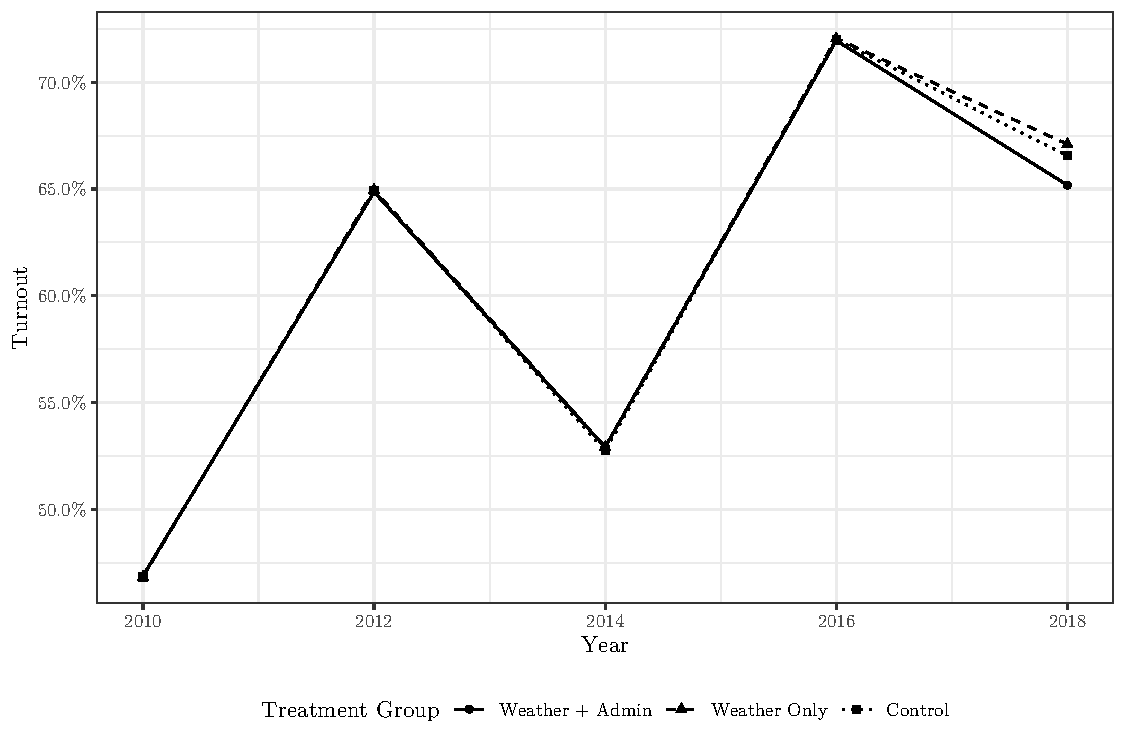
\includegraphics{hurricane_michael_files/figure-latex/tripd-to-chunk-1} 

}

\caption{\label{fig:trip-diff-plot}General Election Turnout for Untreated Voters, Voters Treated by Weather, and Voters Treated by Weather and Administrative Changes, 2010--2018}\label{fig:tripd-to-chunk}
\end{figure}

Disentangling the administrative and weather effects of the storm requires the estimation of the triple-differences model. This model is estimated by Equation (1). In the model, \emph{Weather Treatment\textsubscript{i} × 2018\textsubscript{t}} is a time-variant dummy that is 1 in 2018 for voters in the panhandle, and 0 for all other voters and in all other periods. \emph{Administrative Treatment\textsubscript{i} × 2018\textsubscript{t}}, meanwhile, take the value 0 for all observations except in 2018 for voters in the counties covered by the Executive Order.

\begin{gather}
\label{eq:1}
v_{it}=\beta_0 + \beta_1Weather Treatment_{i}\times 2018_{t} + \\ 
\beta_2Administrative Treatment_{i}\times 2018_{t} + \nonumber \\
\delta{County}_{i} + \delta{Year}_{t} + \nonumber \\
\delta{Z}_{it} + \mathcal{E}_{it}. \nonumber
\end{gather}

The estimation strategy, then, takes the form of a two-way fixed effects model. Individual \emph{i}'s turnout (\emph{v}) in year \emph{t} is a function of the year and their location. In the equation, \emph{\(\beta\)\textsubscript{1}} tests the weather effect for the voters treated by the hurricane's weather in 2018, and \emph{\(\beta\)\textsubscript{2}} captures the estimated administrative effect of living in a county covered by the Executive Order, above-and-beyond the effect associated with the weather treatment. The matrices \emph{\(\delta\)County\textsubscript{i}} and \emph{\(\delta\)Year\textsubscript{t}} contain county and year fixed effects, respectively. The matrix \emph{\(\delta\)Z\textsubscript{i}} includes the measures for relative rainfall and polling place closures interacted with year, county, and weather-treatment dummies.

In Figure \ref{fig:trip-diff-coef} we present the results of these models, again fit using an ordinary least squares specification. Although the figure shows only the estimated administrative treatment effects, the full table can be found in the Supplementary Information. In the left-hand panel, we present estimates of the administrative treatment effect without controlling for the treated voters' changed distance to their nearest polling place. The right-hand panel, meanwhile, shows the administrative effect after we control for this key variable. We show the overall estimated treatment effect for the administratively-treated counties as a whole at the top of each panel, followed by the estimated treatment effect for each individual county. The bottom panels are the result of single models, in which each county's estimated treatment effect is shown relative to a null hypothesis of zero treatment effect, rather than a null hypothesis of zero difference from the reference treated county.

\begin{figure}[h]

{\centering 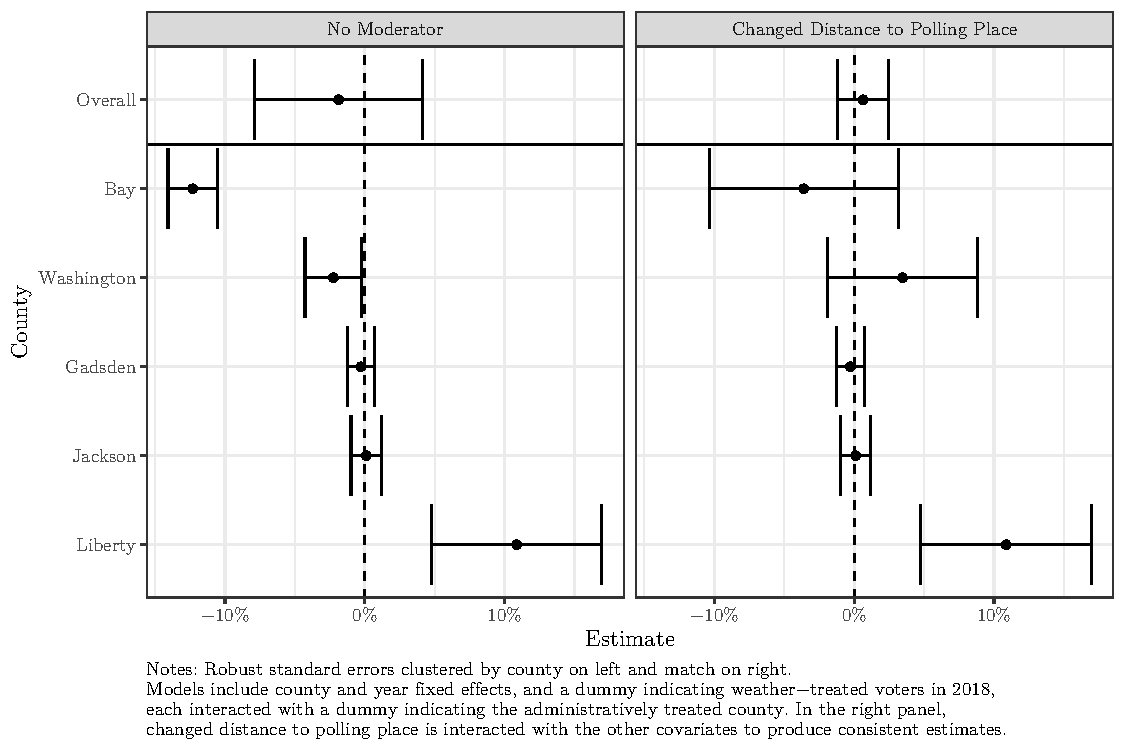
\includegraphics{hurricane_michael_files/figure-latex/tripd-to-chunk-reg-1} 

}

\caption{\label{fig:trip-diff-coef}Estimated Adminsitrative Treatment Effects}\label{fig:tripd-to-chunk-reg}
\end{figure}

Figure \ref{fig:trip-diff-coef} makes a number of things clear. First, neither model estimates a statistically significant treatment effect for the treated counties \emph{as a whole}, although each individual county's treatment effect is significantly different than 0. This provides further corroboration for the notion that what mattered in the Panhandle in 2018 was how each individual county exercised its latitude under the Executive Order, \emph{not} the Executive Order as a single, monolithic treatment.

Secondly, as we move from the left-hand to right-hand panels, we see that the bulk of the administrative treatment is explained by the polling place consolidation. For Bay County, for instance, the point estimate is halved and the estimated effect is statistically nonsignificant. The administrative treatment effect actually becomes positive for Washington County once we control for the effect of these closed polling places, and the estimated effects in Gadsden and Liberty County remain minuscule and are statistically nonsignificant. The large effect in Liberty County likely reflects both the county's ability to keep polling places in this area open, and the relatively poor weather in the buffer.

Although Liberty County voters in the buffer were subjected to worse weather than any of the others (rainfall for Liberty County voters was 229\% of normal, compared with 131\%, 140\%, 155\%, and 213\% for Washington, Jackson, Bay, and Gadsden Counties, respectively), the county kept all its polling places open. The presence of adverse weather may have created more space for the other administrative changes allowed under the Executive Order to ``recoup'' lost turnout due to the storm; indeed, as we show in the Supplementary Information, the weather treatment for the matched voters just outside of Liberty County was in fact severely depressed relative to voters elsewhere in the state.

\hypertarget{shifting-vote-modes}{%
\section*{Shifting Vote Modes}\label{shifting-vote-modes}}
\addcontentsline{toc}{section}{Shifting Vote Modes}

Having established that turnout was substantially depressed in the treated counties and that a non-trivial amount of the depression arose from administrative costs, we turn to a new question: did the storm shift \emph{how} people cast their ballots? Fujiwara and colleagues (\protect\hyperlink{ref-Fujiwara2016}{2016}) find rain disrupts the habit forming nature of voting, but do not consider convenience voting. We know that Executive Order 18-283 loosened restrictions on early and mail balloting; we therefore expect that, relative to the rest of the state, a higher share of ballots in the treated counties cast their ballots in one of these ways.

We return to the matches produced earlier in this paper, where every voter in the treated counties was matched with five voters elsewhere in the state. Figure \ref{fig:vote-mode} demonstrates the share of registered voters that cast a ballot either at the polling place, early in person, or absentee in each general election from the past decade. In each case, the denominator is the number of registered voters in 2018. Figure \ref{fig:vote-mode} makes clear that the decline in turnout was a product of lower turnout on election day and via absentee voting, while it seems that early voting was higher in the treated counties due to Hurricane Michael.

\begin{figure}[h]

{\centering 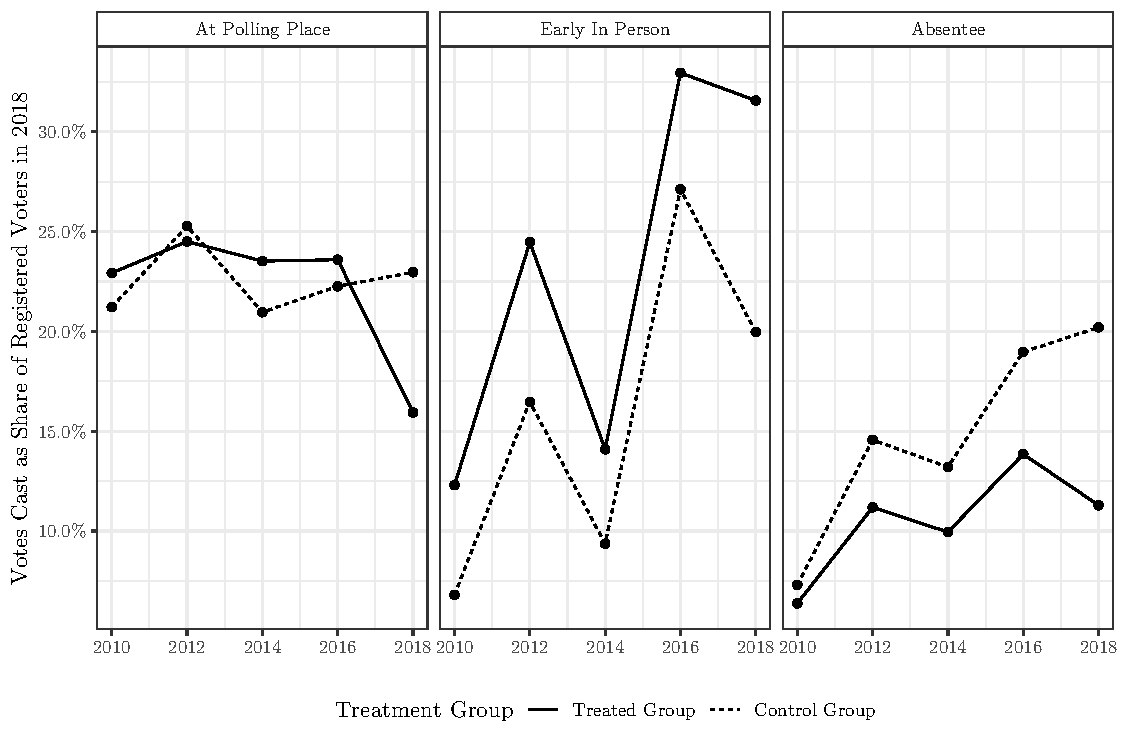
\includegraphics{hurricane_michael_files/figure-latex/vote-mode-chunk-1} 

}

\caption{\label{fig:vote-mode}Average Marginal Effect of Hurricane Michael on Vote Mode}\label{fig:vote-mode-chunk}
\end{figure}

To more directly estimate the effect of Hurricane Michael and the polling place closures allowed under the Executive Order on vote-mode, we measure how far each treated voter lived from the closest planned polling place and the polling place that actually opened on election day. Using a multinomial logistic regression, we test whether increasing the difference between these distances was related to vote-mode or abstention in 2018. In addition to the difference between expected and actual distance to the closest polling place, we include other covariates. We measure how far a voter lived from her closest \emph{planned} polling place, in case voters in more remote parts of the counties generally voted differently in 2018 than other voters. We control for individual characteristics such as race, age, and partisan affiliation. We also include dummies indicating how (or whether) each voter participated in the 2010--2016 general elections. While we include all the voters in each of the covered counties, this set-up will primarily test effects in the counties that saw the most consolidation; voters in counties where few polling places were closed will see little-to-no difference between the planned and actual distance to a polling place.

Because the coefficients from the mulinomial logistic regression are difficult to interpret on their own, we include here the marginal effects plots from this model (the full regression table can be found in the Supplementary Information). Figure \ref{fig:marg-multi} presents the marginal effect of the change in distance to the nearest polling place on vote method while keeping all other covariates in the model at their means.

\begin{figure}[h]

{\centering 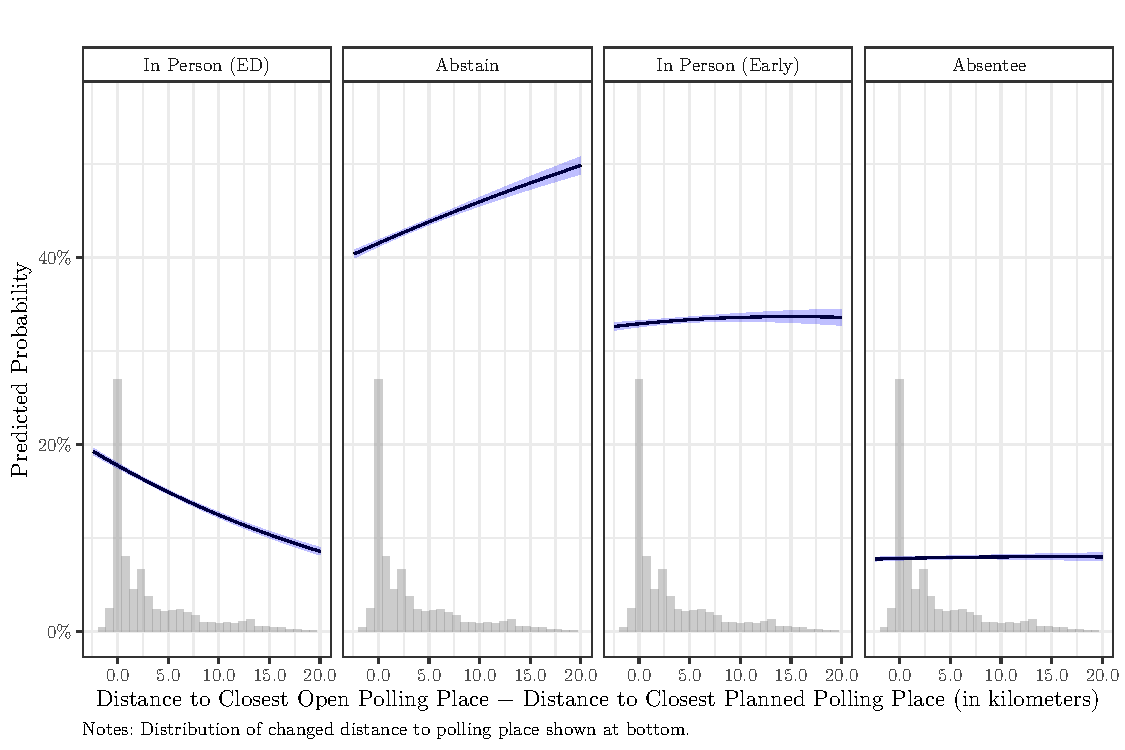
\includegraphics{hurricane_michael_files/figure-latex/marg-multi-1} 

}

\caption{\label{fig:marg-multi}Marginal Effect of Changed Distance to Polling Place on 2018 Vote Mode}\label{fig:marg-multi}
\end{figure}

Figure \ref{fig:marg-multi} indicates that, as voters suddenly had to travel further to the nearest polling place, they were substantially less likely to vote in person on election day (``In Person (ED)''). The bulk of these voters \emph{did not} shift to absentee voting or early in-person voting; rather, they were much more likely to abstain from casting a ballot at all. Thus, although administrators took steps to make early and mail voting easier, these efforts were not particularly effective at offsetting the costs associated with polling place consolidation.

\hypertarget{discussion-and-conclusion}{%
\section*{Discussion and Conclusion}\label{discussion-and-conclusion}}
\addcontentsline{toc}{section}{Discussion and Conclusion}

Election Day in the United States consistently falls near the end of hurricane season. Superstorm Sandy struck New York and New Jersey just days before the midterm elections in 2012, wreaking immense havoc. Hurricane Matthew struck the Southeastern United States weeks before the 2016 presidential election, killing dozens and causing more than \$2.5 billion in damages. And in October of 2018---less than a month before the highest-turnout midterm election in a century---Hurricane Michael made landfall. \protect\hyperlink{ref-Mann2006}{Mann and Emanuel} (\protect\hyperlink{ref-Mann2006}{2006}) and others have linked Atlantic hurricanes to climate change, indicating that these disruptions to election day activity are likely to increase in coming years. Understanding how storms of this nature impact turnout---and whether election administrators' responses are sufficient to avoid depressed turnout---is therefore vitally important, particularly in swing states such as Florida and North Carolina that are subject to severe coastal natural disasters.

As this paper demonstrates, Florida's response to Hurricane Michael was only somewhat effective: although Governor Scott allowed for increased access to early and mail voting in eight counties, mail balloting use in these areas actually \emph{dropped} relative to the rest of the state (see Figure \ref{fig:vote-mode}). Despite the Executive Order, turnout dropped substantially for voters who suddenly were faced with long distances to the closest polling places. These voters did not move to vote-by-mail options in appreciable numbers. This cannot be attributed solely to the weather: even after decomposing the weather and administrative effects of the storm, we find there were substantial negative administrative effects for the region as a whole.

This overall administrative effect, however, masks considerable heterogeneity at the county level. Counties that did not close their polling places saw negligible or even positive turnout effects. These results demonstrate the importance of polling place locations, even in the context of permissive convenience voting. Loosening restrictions on where mail ballots could be sent and how they could be returned had little effect on the use of mail ballots in the election in counties with major polling place closures. Without the Executive Order, polling places would still have been moved because some had been destroyed, but the discretion granted to reduce the number of polling places apparently substantially reduced turnout. Thus, the Executive Order likely increased the administrative costs of voting where polling places were closed.

The data at hand cannot explain why the polling place closures resulted in such extensive turnout reductions, and why the loosened provisions granted under the Executive Order did not recoup these losses. The timing of the Executive Order, however, might shed some light. Although the hurricane made landfall on October 10, the Executive Order was not signed until more than a week later, on October 18---fewer than three weeks before the November 6 general election. This left little time for an effective public education campaign, perhaps limiting the number of voters who learned and took advantage of the changed rules. We found very few news articles detailing the changes and making the information easily available to voters (but see \protect\hyperlink{ref-WJHG2018}{\emph{WJHG - Panama City} 2018}; \protect\hyperlink{ref-Vasquez2018}{Vasquez 2018}; \protect\hyperlink{ref-McDonald2018}{McDonald 2018}; \protect\hyperlink{ref-Fineout2018}{Fineout 2018}), and what information did get published often listed only relocated polling places with no information about loosened mail voting restrictions (see, for instance, \protect\hyperlink{ref-gadsdentimes2018}{\emph{Gadsden Times} 2018}). It is possible, of course, that local televised news communicated the changes to viewers; however, based on our search of published information, that information would have been difficult to find for voters who missed the televised news. We found no evidence that the \emph{Florida Times-Union} (the largest paper in Northern Florida) or the \emph{Tampa Bay Times} (the largest paper in the state) published any articles detailing the changes brought about by the Executive Order.

Natural disasters cause immense disruptions in the lives of Americans, and these effects will only grow in the coming decades. Loss of life and loss of property are devastating enough---they should not be accompanied by the loss of the franchise as well. As this study demonstrates, election administrators can avoid inadvertently curtailing access to the ballot box by maintaining in-person voting options and easing other restrictions. Managing elections is a difficult job under even the best of circumstances; this is surely even more true in the fact of natural disasters. Nevertheless, this article joins a growing body of research articulating the central importance of keeping polling places open.

\newpage

\hypertarget{references}{%
\section*{References}\label{references}}
\addcontentsline{toc}{section}{References}

\hypertarget{refs}{}
\begin{CSLReferences}{1}{0}
\leavevmode\hypertarget{ref-Abadie2020}{}%
Abadie, Alberto, and Jann Spiess. 2020. {``Robust {Post}-{Matching Inference}.''} \emph{Journal of the American Statistical Association} 0 (0): 1--13. \url{https://doi.org/10.1080/01621459.2020.1840383}.

\leavevmode\hypertarget{ref-Brady2011}{}%
Brady, Henry, and John McNulty. 2011. {``Turning Out to Vote: {The Costs} of {Finding} and {Getting} to the {Polling Place}.''} \emph{American Political Science Review} 105 (1): 115--34.

\leavevmode\hypertarget{ref-Brown2019}{}%
Brown, Mitchell, Kathleen Hale, and Bridgett King. 2019. \emph{The {Future} of {Election Administration}: {Cases} and {Conversations}}. {Palgrave Macmillan}.

\leavevmode\hypertarget{ref-Burden2014}{}%
Burden, Barry C., David T. Canon, Kenneth R. Mayer, and Donald P. Moynihan. 2014. {``Election {Laws}, {Mobilization}, and {Turnout}: {The Unanticipated Consequences} of {Election Reform}.''} \emph{American Journal of Political Science} 58 (1): 95--109. \url{https://doi.org/10.1111/ajps.12063}.

\leavevmode\hypertarget{ref-Cantoni2020}{}%
Cantoni, Enrico. 2020. {``A {Precinct Too Far}: {Turnout} and {Voting Costs}.''} \emph{American Economic Journal: Applied Economics} 12 (1): 61--85.

\leavevmode\hypertarget{ref-Chamberlain2021}{}%
Chamberlain, Scott. 2021. \emph{Rnoaa: '{NOAA}' {Weather Data} from {R}}. \url{https://CRAN.R-project.org/package=rnoaa}.

\leavevmode\hypertarget{ref-Cooperman2017}{}%
Cooperman, Alicia. 2017. {``Randomization {Inference} with {Rainfall Data}: {Using Historical Weather Patterns} for {Variance Estimation}.''} \emph{Political Analysis} 25 (3): 277--88.

\leavevmode\hypertarget{ref-Dyck2005}{}%
Dyck, Joshua, and James Gimpel. 2005. {``Distance, {Turnout}, and the {Convenience} of {Voting}.''} \emph{Social Science Quarterly} 86 (3): 531--48.

\leavevmode\hypertarget{ref-Fineout2018}{}%
Fineout, Gary. 2018. {``Florida to Bend Voting Rules in Counties Hit by Hurricane.''} \emph{Northwest Florida Daily News}, October 18, 2018. \url{https://www.nwfdailynews.com/news/20181018/florida-to-bend-voting-rules-in-counties-hit-by-hurricane}.

\leavevmode\hypertarget{ref-Fraga2010}{}%
Fraga, Bernard, and Eitan Hersh. 2010. {``Voting {Costs} and {Voter Turnout} in {Competitive Elections}.''} \emph{Quarterly Journal of Political Science} 5: 339--56. https://doi.org/\url{http://dx.doi.org/10.1561/100.00010093_supp}.

\leavevmode\hypertarget{ref-Fujiwara2016}{}%
Fujiwara, Thomas, Kyle Meng, and Tom Vogl. 2016. {``Habit {Formation} in {Voting}: {Evidence} from {Rainy Elections}.''} \emph{American Economic Journal: Applied Economics} 8 (4): 160--88.

\leavevmode\hypertarget{ref-gadsdentimes2018}{}%
\emph{Gadsden Times}. 2018. {``Changes in Polling Places at Three Locations,''} October 30, 2018. \url{https://www.gadsdentimes.com/news/20181030/changes-in-polling-places-at-three-locations}.

\leavevmode\hypertarget{ref-Garcia-Rodriguez2020}{}%
Garcia-Rodriguez, Abian, and Paul Redmond. 2020. {``Rainfall, Population Density and Voter Turnout.''} \emph{Electoral Studies} 64 (April): 102128. \url{https://doi.org/10.1016/j.electstud.2020.102128}.

\leavevmode\hypertarget{ref-Gatrell2002}{}%
Gatrell, Jay, and Gregory Bierly. 2002. {``Weather and {Voter Turnout}: {Kentucky Primary} and {General Elections}, 1990-2000.''} \emph{Southeastern Geographer} 42 (1): 114--34.

\leavevmode\hypertarget{ref-Hale2015}{}%
Hale, Kathleen, Robert Montjoy, and Mitchell Brown. 2015. \emph{Administering {Elections}}. {Palgrave Macmillan}.

\leavevmode\hypertarget{ref-Hansford2010}{}%
Hansford, Thomas, and Brad Gomez. 2010. {``Estimating the {Electoral Effects} of {Voter Turnout}.''} \emph{American Political Science Review} 104: 268--88.

\leavevmode\hypertarget{ref-Haspel2005}{}%
Haspel, Moshe, and H. Gibbs Knotts. 2005. {``Location, {Location}, {Location}: {Precinct Placement} and the {Costs} of {Voting}.''} \emph{Journal of Politics} 67 (2): 560--73.

\leavevmode\hypertarget{ref-Imai2020}{}%
Imai, Kosuke, In Song Kim, and Erik Wang. 2020. {``Matching {Methods} for {Causal Inference} with {Time}-{Series Cross}-{Sectional Data}.''} \emph{Working Paper}. \url{https://doi.org/Matching\%20Methods\%20for\%20Causal\%20Inference\%20with\%20Time-Series\%20Cross-Sectional\%20Data}.

\leavevmode\hypertarget{ref-Kaplan2020}{}%
Kaplan, Ethan, and Haishan Yuan. 2020. {``Early {Voting Laws}, {Voter Turnout}, and {Partisan Vote Composition}: {Evidence} from {Ohio}.''} \emph{American Economic Journal: Applied Economics} 12 (1): 32--60.

\leavevmode\hypertarget{ref-Keele2015b}{}%
Keele, Luke, and Rocío Titiunik. 2015. {``Geographic {Boundaries} as {Regression Discontinuities}.''} \emph{Political Analysis} 23 (1): 127--55. \url{https://doi.org/10.1093/pan/mpu014}.

\leavevmode\hypertarget{ref-Keele2015a}{}%
Keele, Luke, Rocío Titiunik, and José R. Zubizarreta. 2015. {``Enhancing a Geographic Regression Discontinuity Design Through Matching to Estimate the Effect of Ballot Initiatives on Voter Turnout.''} \emph{Journal of the Royal Statistical Society: Series A (Statistics in Society)} 178 (1): 223--39. \url{https://doi.org/10.1111/rssa.12056}.

\leavevmode\hypertarget{ref-Kitamura2021}{}%
Kitamura, Shuhei, and Tetsuya Matsubayashi. 2021. {``Dynamic {Voting}.''} \emph{Working Paper}, January. \url{https://doi.org/10.2139/ssrn.3630064}.

\leavevmode\hypertarget{ref-Kropf2012}{}%
Kropf, Martha, and David Kimball. 2012. \emph{Helping {America Vote}: {The Limits} of {Election Reform}}. {New York}: {Routledge}.

\leavevmode\hypertarget{ref-Larocca2011}{}%
Larocca, Roger, and John S. Klemanski. 2011. {``U.{S}. {State Election Reform} and {Turnout} in {Presidential Elections}.''} \emph{State Politics \& Policy Quarterly} 11 (1): 76--101. \url{https://doi.org/10.1177/1532440010387401}.

\leavevmode\hypertarget{ref-Lasala-Blanco2017}{}%
Lasala-Blanco, Narayani, Robert Shapiro, and Viviana Rivera-Burgos. 2017. {``Turnout and {Weather Disruptions}: {Survey Evidence} from the 2012 {Presidential Elections} in the {Aftermath} of {Hurricane Sandy}.''} \emph{Electoral Studies} 45: 141--52.

\leavevmode\hypertarget{ref-Macias2020}{}%
Macías, Raúl, and Myrna Pérez. 2020. {``Voters {Need Safe} and {Sanitary In}-{Person Voting Options}.''} {Brennan Center for Justice}. \url{https://www.brennancenter.org/our-work/research-reports/voters-need-safe-and-sanitary-person-voting-options}.

\leavevmode\hypertarget{ref-Mann2006}{}%
Mann, Michael E., and Kerry A. Emanuel. 2006. {``Atlantic Hurricane Trends Linked to Climate Change.''} \emph{Eos, Transactions American Geophysical Union} 87 (24): 233--41. \url{https://doi.org/10.1029/2006EO240001}.

\leavevmode\hypertarget{ref-McDonald2018}{}%
McDonald, Zack. 2018. {``Bay Voters Getting 5 'Mega Voting' Sites.''} \emph{Panama City News Herald}, October 23, 2018. \url{https://www.newsherald.com/news/20181023/bay-voters-getting-5-mega-voting-sites}.

\leavevmode\hypertarget{ref-McNulty2009}{}%
McNulty, John, Conor Dowling, and Margaret Ariotti. 2009. {``Driving {Saints} to {Sin}: {How Increasing} the {Difficulty} of {Voting Dissuades Even} the {Most Motivated Voters}.''} \emph{Political Analysis} 17 (4): 435--55.

\leavevmode\hypertarget{ref-Morris2021}{}%
Morris, Kevin, and Peter Miller. 2021. {``Voting in a {Pandemic}: {COVID}-19 and {Primary Turnout} in {Milwaukee}, {Wisconsin}.''} \emph{Urban Affairs Review}, April, 10780874211005016. \url{https://doi.org/10.1177/10780874211005016}.

\leavevmode\hypertarget{ref-Nyhan2017}{}%
Nyhan, Brendan, Christopher Skovron, and Rocío Titiunik. 2017. {``Differential {Registration Bias} in {Voter File Data}: {A Sensitivity Analysis Approach}.''} \emph{American Journal of Political Science} 61 (3): 744--60. \url{https://doi.org/10.1111/ajps.12288}.

\leavevmode\hypertarget{ref-Parks2018}{}%
Parks, Miles. 2018. {``After {Hurricane Michael}, {Voting} '{Is The Last Thing On Their Minds}'.''} \emph{NPR.org}, October 25, 2018. \url{https://www.npr.org/2018/10/25/659819848/after-hurricane-michael-voting-is-the-last-thing-on-their-minds}.

\leavevmode\hypertarget{ref-Persson2014}{}%
Persson, Mikael, Anders Sundell, and Richard Öhrvall. 2014. {``Does {Election Day Weather Affect Voter Turnout}? {Evidence} from {Swedish Elections}.''} \emph{Electoral Studies} 33: 335--42.

\leavevmode\hypertarget{ref-Rallings2003}{}%
Rallings, Colin, Michael Thrasher, and Roman Borisyuk. 2003. {``Seasonal {Factors}, Voter Fatigue, and the Costs of Voting.''} \emph{Electoral Studies} 22: 65--79.

\leavevmode\hypertarget{ref-Ricardson1996}{}%
Ricardson, Lilliard, and Grant Neeley. 1996. {``The {Impact} of {Early Voting} on {Turnout}: {The} 1994 {Elections} in {Tennessee}.''} \emph{State \& Local Government Review} 28 (3): 173--79.

\leavevmode\hypertarget{ref-Root2020}{}%
Root, Danielle, Danyelle Solomon, Rebecca Cokley, Tori O'Neal, Jamal R. Watkins, and Dominik Whitehead. 2020. {``In {Expanding Vote} by {Mail}, {States Must Maintain In}-{Person Voting Options During} the {Coronavirus Pandemic}.''} {Center for American Progress}. \url{https://www.americanprogress.org/issues/democracy/news/2020/04/20/483438/expanding-vote-mail-states-must-maintain-person-voting-options-coronavirus-pandemic/}.

\leavevmode\hypertarget{ref-Sekhon2009}{}%
Sekhon, Jasjeet. 2009. {``Opiates for the {Matches}: {Matching Methods} for {Causal Inference}.''} \emph{Annual Review of Political Science} 12: 487--508.

\leavevmode\hypertarget{ref-Sekhon2011}{}%
---------. 2011. {``Multivariate and {Propensity Score Matching Software} with {Automated Balance Optimization}: {The Matching} Package for {R}.''} \emph{Journal of Statistical Software} 42 (1): 1--52. \url{https://doi.org/10.18637/jss.v042.i07}.

\leavevmode\hypertarget{ref-Stein2015}{}%
Stein, Robert. 2015. {``Election {Administration During National Disasters} and {Emergencies}: {Hurricane Sandy} and the 2012 {Election}.''} \emph{Election Law Journal} 14: 66--73.

\leavevmode\hypertarget{ref-Vasquez2018}{}%
Vasquez, Savannah. 2018. {``{HURRICANE MICHAEL}: {How} to Vote in {Gulf County}.''} \emph{The Star}, October 18, 2018. \url{https://www.starfl.com/news/20181018/hurricane-michael-how-to-vote-in-gulf-county}.

\leavevmode\hypertarget{ref-Velez2013}{}%
Velez, Yamil, and David Martin. 2013. {``Sandy the {Rainmaker}: {The Electoral Impact} of a {Super Storm}.''} \emph{PS: Political Science and Politics} 46: 313--23.

\leavevmode\hypertarget{ref-Walker2019}{}%
Walker, Hannah L., Michael C. Herron, and Daniel A. Smith. 2019. {``Early {Voting Changes} and {Voter Turnout}: {North Carolina} in the 2016 {General Election}.''} \emph{Political Behavior} 41 (4): 841--69. \url{https://doi.org/10.1007/s11109-018-9473-5}.

\leavevmode\hypertarget{ref-WJHG2018}{}%
\emph{WJHG - Panama City}. 2018. {``Bay {County Hurricane Michael Recovery Information},''} October 31, 2018. \url{https://www.wjhg.com/content/news/Bay-County--498037961.html}.

\end{CSLReferences}

\end{document}
